\subsection{Konvektion}
\label{section:convection}
I fasta ämnen går det utmärkt att approximera värmeflöde enbart med hjälp
av värmeledningsekvationen. Detta håller dock ej lika bra för fluider, det vill säga
material som deformeras då de utsätts för tryck.
Under dessa förhållanden
måste det tas hänsyn till konservation av massa, energi samt rörelsemoment.
I det följande kommer en homogen fluid betraktas. För att härleda giltiga differentialekvationer som beskriver en fluids rörelse används ofta sambandet

\begin{equation}
\label{eq:convection:reynolds}
\frac{dB}{dt} = \frac{d}{dt}\left( \int_{V} \frac{dB}{dm} \rho dV \right) + \int_{\partial V} \frac{dB}{dm} \rho \left( \mathbf{v} \cdot \mathbf{n} \right)dA,
\end{equation}

där $B$ är en godtycklig egenskap av fluiden, exempelvis dess rörelsemängd, V är den så kallade kontrollvolymen (omfattande ett godtyckligt valt område), $\partial V$ är denna kontrollvolyms rand, $\rho$ är fluidens densitet, $\mathbf{v}$ är fluidens hastighetsvektor och $\mathbf{n}$ är normalvektorn till randen. Detta samband benämns vanligen Reynolds transportteorem\footnote{För närmare beskrivning och härledning, se White, 2011 \cite{white11}}.

Sätt $B = m$ där $m$ är fluidens massa (oberoende av tiden) och låt $V$ vara en tidsoberoende volym. Ett uttryck för masskonservering erhålls:

\begin{equation}
\label{eq:convection:masscon}
\int_V \frac{\partial \rho}{\partial t} dV + \int_{\partial V} \rho \left( \mathbf{v} \cdot \mathbf{n} \right) dA = 0
\end{equation}

Första termen i detta uttryck beskriver förändringar i densiteten inom kontrollvolymen medan andra termen omfattar alla flöden in och ut genom kontrollvolymens rand. För masskonservering krävs alltså att summan av dessa termer ska vara noll. Den andra termen kan, vid diskreta flödesmängder, även skrivas som

\begin{equation}
\label{eq:convection:discrete}
\int_{\partial V} \rho \left( \mathbf{v} \cdot \mathbf{n} \right) dA = \sum_i \left( \rho \mathbf{v}_i\cdot \mathbf{A}_i \right)_{ut} - \sum_i \left( \rho \mathbf{v}_i\cdot \mathbf{A}_i \right)_{in}
\end{equation}

\begin{figure}[hpbt]
\centering
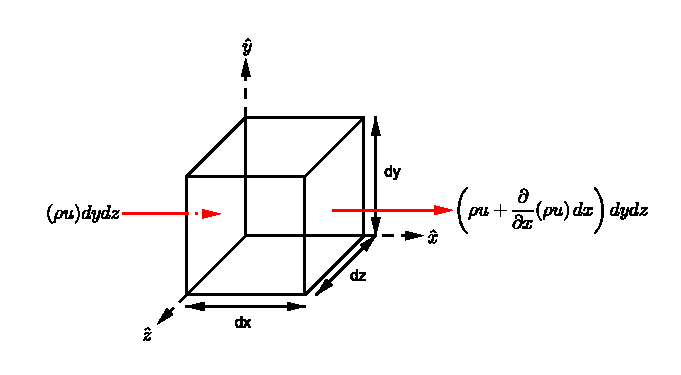
\includegraphics[scale=1]{images/massflowcube.eps}
\caption{\label{fig:massflowcube} Infinitesimal kontrollvolym för derivering av bevaranderelationer, här med massflödet exemplifierat}
\end{figure}

Betrakta nu en infinitesimal kontrollvolym som den i figur \ref{fig:massflowcube}. In- och utflödena kan här approximeras till endimensionella flöden och \eqref{eq:convection:masscon} reduceras till

\begin{equation}
\label{eq:convection:massconinf}
\int_V \frac{\partial \rho}{\partial t} dxdydz + \frac{\partial}{\partial x}\left( \rho u \right)dxdydz + \frac{\partial}{\partial y}\left( \rho v \right)dxdydz + \frac{\partial}{\partial z}\left( \rho w \right)dxdydz = 0
\end{equation}

vilket, om dxdydz tas bort, kan förenklas som

\begin{equation}
\label{eq:convection:continuity}
\frac{\partial \rho}{\partial t} + \nabla \cdot \left( \rho \mathbf{v} \right) = 0
\end{equation}

Om inkompressibilitet antas ($\rho$ = konstant) reduceras denna ekvation ytterligare till

\begin{equation}
\label{eq:convection:continuityinc}
\nabla \cdot \mathbf{v} = 0
\end{equation}

Detta är kontinuitetsekvationen för inkompressibla fluider.

Betrakta åter \eqref{eq:convection:reynolds} och sätt nu $B = m\mathbf{v}$. På samma vis som kontinuitetsekvationen \eqref{eq:convection:continuityinc} härleddes, fås för det infinitesimala volymelementet i figur sambandet

\begin{eqnarray}
\label{eq:convection:linear}
\sum \mathbf{F} & = & \frac{\partial}{\partial t} \left( \int_V \mathbf{v} \rho dV \right) + \sum_i \left( \dot{m}_i \mathbf{v}_i \right)_{ut} - \sum_i \left( \dot{m}_i \mathbf{v}_i \right)_{in}\nonumber\\
& = &\left(\frac{\partial}{\partial t} \left( \rho\mathbf{v} \right) + \frac{\partial}{\partial x}\left( \rho u \mathbf{v}\right) + \frac{\partial}{\partial y}\left( \rho v \mathbf{v}\right) + \frac{\partial}{\partial z}\left( \rho w \mathbf{v}\right)\right)dxdydz
\end{eqnarray}

ty enligt Newtons andra lag är tidsderivatan av rörelsemängden $m\mathbf{v}$ lika med summan av alla krafter som verkar på kroppen. $\dot{m}_i$ betecknar här massflödet $\rho\mathbf{v}_i\cdot\mathbf{A}_i$.

Det sista högerledet kan skrivas om som

\begin{equation}
\left( \mathbf{v}\left[ \frac{\partial \rho}{\partial t} + \nabla\cdot \rho \mathbf{v}\right] + \rho\left[ \frac{\partial \mathbf{v}}{\partial t} + u\frac{\partial\mathbf{v}}{\partial x} + v\frac{\partial\mathbf{v}}{\partial y} + w\frac{\partial\mathbf{v}}{\partial z} \right]\right)dxdydz.
\end{equation}

Första termen inom hakparentes är kontinuitetsekvationen \eqref{eq:convection:continuity} och går alltså bort.
\begin{comment}
Den andra hakparentesen motsvarar något som kallas materiederivata. Man kan visa att 

% OBS, blandat tensorer och vektorer
\begin{equation}
\label{eq:convection:material}
\frac{d\mathbf{v}}{dt} = \frac{\partial \mathbf{v}}{\partial t} + \mathbf{v}_i\frac{\partial \mathbf{v}}{\partial x_i}
\end{equation}

och därmed reduceras \eqref{eq:convection:linear} till

\begin{equation}
\label{eq:convection:linearfinal}
\sum \mathbf{F} = \rho \frac{d\mathbf{v}}{dt}dxdydz.
\end{equation}
\end{comment}

Därmed reduceras \eqref{eq:convection:linear} till

\begin{equation}
\label{eq:convection:linearfinal}
\sum \mathbf{F} = \rho \left( \frac{\partial \mathbf{v}}{\partial t} + \mathbf{v}\cdot \nabla\mathbf{v} \right)dxdydz.
\end{equation}

Summan av de på volymen verkande krafterna måste nu utvecklas. Dessa krafter uppstår på grund av gravitation, tryck och viskositet. Andra krafter, såsom från elektromagnetiska fält, kan i sammanhanget anses vara försumbara. Gravitationskraften $\mathbf{F}_g$ beskrivs för den infinitesimala volymen med $\rho \mathbf{g} dxdydz = \rho g dxdydz \hat{z}$. Tryckkraften $\mathbf{F}_p$, i sin tur, ges av tryckgradienten $-\nabla \left( p \right) dxdydz$. Viskösa kraften $\mathbf{F}_{visc}$ är lite besvärligare att sammanställa. Anta att volymen är en Newtonsk fluid, det vill säga stresstensorn $\tau$ är linjärt proportionell mot hastighetsgradienten $\nabla\mathbf{v}$ med proportionaltitetskonstanten $\mu$, $\tau = \mu \nabla \mathbf{v}$. Den viskösa kraften verkande på kroppen blir då $\mathbf{F}_{visc} = \mu\Delta\mathbf{v}dxdydz$.

% Skriv om till integralrelationer och använd gauss sats, därefter infinitesimal volym

Vi har alltså ekvationssystemet

\begin{eqnarray}
\label{eq:convection:momentum}
\rho\left(\frac{\partial u}{\partial t} + \mathbf{v}\cdot \nabla u\right) & = & -\frac{\partial p}{\partial x} + \mu\Delta u \nonumber\\
\rho\left(\frac{\partial v}{\partial t} + \mathbf{v}\cdot \nabla v\right) & = & -\frac{\partial p}{\partial y} + \mu\Delta v\\
\rho\left(\frac{\partial w}{\partial t} + \mathbf{v}\cdot \nabla w\right) & = & -\rho g -\frac{\partial p}{\partial z} + \mu\Delta w\nonumber
\end{eqnarray}

% Energirelationen

För homogena inkompressibla fluider i två dimensioner gäller då ekvationerna
\eqref{eq:convection:continuity}, \eqref{eq:convection:momentum} samt \eqref{eq:convection:energy}. Här
är $\mathbf{v} = (u,w)$ hastighetsvektorn, $\alpha$ är den termiska
diffusiviteten, $\nu$ är den kinematiska viskositeten, $p$ är trycket,
$\rho$ är densiteten, $g$ är den lokala tyngdaccelerationen
och slutligen är $\rho_0$ referensdensiteten.

% Denna kallas för convection-diffusion equation
% Kan härledas mha kontinuitetsekvationen och Ficks lag
\begin{equation}
\label{eq:convection:energy}
\frac{\partial T}{\partial t} + \mathbf{v}\cdot\nabla T = \alpha\Delta T
\end{equation}

\subsubsection{Boussinesq approximation}

För flytkraftsdrivet flöde kan det vara lämpligt att använda sig av
Boussinesq approximation. Denna säger att det enda som påverkar trycket är
tyngdaccelerationen. Genom detta är det möjligt att sätta upp uttryck för densiteten
och tryckderivatorna enligt ekvationerna \eqref{eq:convection:density}
och \eqref{eq:convection:pressurez}. Här är
$\beta$ den volymetriska expansionskonstanten och
$T_0$ temperaturen som råder vid referensdensiteten $\rho_0$.

\begin{equation}
\label{eq:convection:density}
\rho = \rho_0[1-\beta(T-T_0)]
\end{equation}

\begin{equation}
\label{eq:convection:pressurez}
\frac{\partial p}{\partial z} = -\rho_0g
\end{equation}


